% mainfile: ../../main.tex
\setchapterpreamble[u]{\margintoc}
\chapter{Supplementary to Part \ref{part:setup}: Optical coupling and vibrations}\label{ch:app:setup}
In this appendix, I give additional information on the optical coupling efficiency of the confocal microscope described in \cref{ch:setup:optics} as well as the knife-edge measurement used to calibrate the optical vibration spectroscopy technique presented in \cref{ch:setup:vibrations}.

\section{Optical coupling}\label{sec:app:setup:optics}
\subsection{Collection efficiency}\label{subsec:app:setup:optics:collection}
In this subsection, I derive the expression for the collection efficiency $\eta_{\mr{c}}$, \cref{eq:setup:optics:coupling:efficiency:collection}, for radiation emitted from a dipole oriented in-plane inside a semiconductor \gls{qw} with refractive index $n$ and collected with a lens of a given \gls{na}.
The dipole fields in spherical coordinates $(r, \vartheta, \varphi)$ in the coordinate system $(z, x, y)$ are given in \cref{eq:setup:optics:coupling:dipole:efield,eq:setup:optics:coupling:dipole:hfield}.\sidenote{
    That is,
    \begin{align*}
        z &= r\sin\vartheta\sin\varphi \\
        x &= r\sin\vartheta\cos\varphi \\
        y &= r\cos\vartheta.
    \end{align*}
}
Since we observe the dipole from the side, \ie, perpendicular to its axis, it is useful to rotate the spherical coordinates $(r, \vartheta, \varphi) \to (r, \theta, \phi)$ aligned with the cartesian coordinate system $(x, y, z)$ in \cref{fig:setup:optics:coupling:emission}.
To this end, observe that with the spherical coordinates
\begin{align}
    x &= r\sin\theta\sin\phi \\
    y &= r\sin\theta\cos\phi \\
    z &= r\cos\theta
\end{align}
we can express the angles in the dipole coordinate system, $(\vartheta, \varphi)$, in terms of angles of the sample coordinate system, $(\theta, \phi)$, by
\begin{align}
    \begin{split}\label{eq:app:setup:optics:collection:vartheta}
        \vartheta &= \arctan(\sqrt{z^2 + y^2}/x) \\
                  &= \arctan(\csc\phi\sqrt{\sin^2\phi + \cot^2\theta})
    \end{split} \\
    \begin{split}\label{eq:app:setup:optics:collection:varphi}
        \varphi &= \arctan(y/z) \\
                &= \arctan(\sin\phi\tan\theta).
    \end{split}
\end{align}
The time-averaged Poynting vector, \cref{eq:setup:optics:coupling:poynting}, is then
\begin{equation}
    \begin{split}
        \expval{\bvec{S}(r, \theta, \phi)} &= \frac{1}{2}\re\left[\bvec{E}(r, \vartheta)\times\bvec{H}^{\ast}(r, \vartheta)\right] \\
                                           &= \frac{\abs{\bvec{p}}^2 c k^4}{32\pi^2\epsilon r^2}\sin^2\vartheta \,\ubvec{r} \\
                                           &= \frac{\abs{\bvec{p}}^2 c k^4}{32\pi^2\epsilon r^2}\left[\cos^2\theta + \sin^2\theta\sin^2\phi\right] \ubvec{r}.
    \end{split}
\end{equation}
Evaluating the integral in \cref{eq:setup:optics:coupling:power} for the escape cone angle $\theta_{\mr{m}} = \arcsin(\NA/n)$ thus yields
\begin{equation}
    \begin{split}
        P_{\mr{m}} &= \int_{0}^{\theta_{\mr{m}}}\dd{\theta}\sin\theta\int_{0}^{2\pi}\dd{\phi}\expval{\bvec{S}(r, \theta, \phi)} \\
                   &= \frac{\abs{\bvec{p}}^2 c k^4}{32\pi^2\epsilon r^2}\left[\frac{4\pi}{3} - \frac{\pi}{3 n^3} \left(4n^2 - \NA^2\right)\sqrt{n^2 - \NA^2}\right],
    \end{split}
\end{equation}
whereas the total emitted power is the well-known expression
\begin{equation}
    \begin{split}
        P_{\mr{tot}} &= \int_{0}^{\pi}\dd{\theta}\sin\theta\int_{0}^{2\pi}\dd{\phi}\expval{\bvec{S}(r, \theta, \phi)} \\
                     &= \frac{\abs{\bvec{p}}^2 c k^4}{12\pi\epsilon r^2}.
    \end{split}
\end{equation}
Together, we therefore find
\begin{equation}
    \eta_{\mr{c}} = \frac{P_{\mr{m}}}{P_{\mr{tot}}} = \frac{1}{2} - \frac{1}{8 n^3} \left(4n^2 - \NA^2\right)\sqrt{n^2 - \NA^2}
\end{equation}
as given in the main text.

\subsection{Mode profile}\label{subsec:app:setup:optics:modes}
In this subsection, I derive the electric field of a dipole situated inside a dielectric slab and oriented parallel to the surface outside of the dielectric.
We use the convention of spherical coordinates from the previous subsection and consider the electric field given in \cref{eq:setup:optics:coupling:dipole:efield} in the rotated coordinate system $(r, \theta, \phi)$ by performing the substitutions given in \cref{eq:app:setup:optics:collection:vartheta,eq:app:setup:optics:collection:varphi}, obtaining
\begin{equation}
    \bvec{E}(r, \theta, \phi) = A(r)\left[E_r(r, \theta, \phi)\ubvec{r} + E_{\theta}(r, \theta, \phi)\ubvec{\theta} + E_{\phi}(r, \theta, \phi)\ubvec{\phi}\right]
\end{equation}
with
\begin{align}
    E_r(r, \theta, \phi) &= f_r(k, r)\sin\theta\cos\phi \\
    E_{\theta}(r, \theta, \phi) &= -f_{\vartheta}(k, r)\cos\theta\cos\phi \\
    E_{\phi}(r, \theta, \phi) &= f_{\vartheta}(k, r)\sin\phi
\end{align}
where we defined
\begin{align}
    f_r(k, r) &= -\frac{2\i}{k r} + \frac{2}{k^2 r^2} \\
    f_{\vartheta}(k, r) &= -1 - \frac{\i}{k r} + \frac{1}{k^2 r^2}
\end{align}
for conciseness.
Now, when the electric field impinges on the surface of the slab, two things must be taken into account: first, it gets refracted, meaning that $\bvec{k}$ is transformed according to Snell's law (\cref{eq:setup:optics:coupling:snell}), and second, the transmitted field is modified with the Fresnel transmission coefficients~\cite{Hecht2017}
\begin{align}
    t_s &= \frac{2\sin\theta\sin\theta^\prime}{\sin(\theta + \theta^\prime)} = \frac{2n\cos\theta}{n\cos\theta + \nu(\theta)} \\
    t_p &= \frac{t_s}{\cos(\theta - \theta^\prime)} = \frac{2n\cos\theta}{\cos\theta + n\nu(\theta)}
\end{align}
where $s$ $(p)$ stands for the component perpendicular (parallel) to the plane of incidence and we defined
\begin{equation}
    \nu(\theta) = \sqrt{1 - n^2\sin^2\theta}.
\end{equation}
In fact, $\ubvec{r}$ and $\ubvec{\theta}$ lie in the $p$ plane and $\ubvec{\phi}$ is parallel to $s$ so that transmission through the interface transforms the electric field components as
\begin{align}
    E_r &\to E_r^\prime = t_p E_r = \frac{n^2 f_r(k, r) \left[\sin(\phi + 2\theta) - \sin(\phi - 2\theta)\right]}{2\left[n\nu(\theta) + \cos\theta\right]} \\
    E_\theta &\to E_\theta^\prime = t_p E_\theta = -\frac{2n f_{\vartheta}(k, r)\nu(\theta)\cos\theta\cos\phi}{n\nu(\theta) + \cos\theta} \\
    E_\phi &\to E_\phi^\prime = t_s E_\phi = -\frac{2n f_{\vartheta}(k, r)\cos\theta\sin\phi}{\nu(\theta) + n\cos\theta}.
\end{align}
As it should be, the radial component vanishes in the far field, $kr\gg 1$, and only the transverse field components survive.
Furthermore, since \ubvec{\phi} does not depend on $\theta$, only \ubvec{r} and \ubvec{\theta} transform according to Snell's law on refraction, resulting in
\begin{align}
    \ubvec{r} \to \ubvec{r}^\prime &= \begin{pmatrix}
        \nu(\theta) \cos\phi \\
        \nu(\theta) \sin\phi \\
        - n\sin\theta
    \end{pmatrix} \\
    \ubvec{\theta} \to \ubvec{\theta}^{\prime} &= \begin{pmatrix}
        n \sin\theta\cos\phi \\
        n \sin\theta\sin\phi \\
        \nu(\theta)
    \end{pmatrix}
\end{align}
in the Cartesian basis defined in \cref{fig:setup:optics:coupling:emission}.
Finally, we can evaluate the electric field amplitude outside the slab in the Cartesian basis,
\begin{equation}
    \bvec{E}^\prime(r, \theta, \phi) = A(r) \sum_{i\in\{x, y, z\}} E_i^\prime(r, \theta, \phi)\ubvec{i},
\end{equation}
with
\begin{align}
    E_x^{\prime} &= f_{r}{\left(k,r \right)} n \sin^{2}{\theta} \cos^{2}{\phi} - f_{\vartheta}{\left(k,r \right)} \left[\nu{\left(\theta \right)} \cos^{2}{\phi} \cos{\theta} - \sin^{2}{\phi}\right] \\
    E_y^{\prime} &= \left[f_{r}{\left(k,r \right)} n \sin^{2}{\theta} - f_{\vartheta}{\left(k,r \right)} \left\lbrace\nu{\left(\theta \right)} \cos{\theta} + 1\right\rbrace\right] \sin{\phi} \cos{\phi} \\
    E_z^{\prime} &= \left[f_{r}{\left(k,r \right)} \nu{\left(\theta \right)} + f_{\vartheta}{\left(k,r \right)} n \cos{\theta}\right] \sin{\theta} \cos{\phi}
\end{align}
where we dropped the arguments for conciseness.

In principle, the angle $\Theta$ and radial distance $R$ for the fields outside the slab would need to be modified when keeping the center of the coordinate system at the dipole source.
That is, if we denote the vector from the dipole to the point in the surface where a particular ray exits the slab by $\bvec{r}$ and the vector from that point to the point of observation by $\bvec{r}^{\prime}$, then $\theta = \arccos(d/r)$ and $\theta^{\prime} = \arccos([z-d]/r^{\prime})$, and the spherical coordinate vector $\bvec{R} = \bvec{r} + \bvec{r}^{\prime}$ with polar angle $\Theta$.
Because of refraction, $\theta\neq\theta^{\prime}$ and hence $\bvec{R}$ has norm $R\neq r + r^{\prime}$.
However, outside the slab we are only interested in the far field at the lens where $R,r^{\prime}\gg d,r$ with $d$ the depth of the dipole inside the slab.
Therefore, we can well approximate $\Theta\approx\theta^{\prime}$ and $R\approx r^{\prime}$ when dealing with the absolute value of the field, corresponding to placing the center of the coordinate system right below the surface of the slab.
For the phase, this approximation likely does not hold well as the radius of the spot on the sample, $\rho_{\mr{m}} = d\tan\theta_{\mr{m}}$, is on the order of the wavelength $\lambda = \lambda_0/n$ and hence the phase is not constant across the radius $\rho$, even when observed from the far field.
A more rigorous, likely numerical, treatment would be needed to fully account for this.

\subsection{Fraunhofer diffraction}\label{subsec:app:setup:optics:diffraction}
The beam focused into the \gls{smf}, \cref{eq:setup:optics:coupling:efield:lens}, experiences diffraction at the ocular lens aperture.
Having approximated the beam as circular, we can write the electric field on the screen, \ie, the fiber end face, as~\cite{Hecht2017}
\begin{equation}\label{eq:app:setup:optics:diffraction}
    \tilde{E}(q) = \frac{\abs{\bvec{p}}k^2}{2\epsilon}\exp(\i k z)\int_0^a\dd{\rho}\rho J_0(k\rho q/\foc) E_x(\rho)
\end{equation}
with $E_x(\rho)$ given by \cref{eq:setup:optics:coupling:efield:lens:x} upon substituting $\theta = \arctan(\rho/\fob)$ and $r=\sqrt{\rho^2 + \fob^2}$, and $J_0(x)$ is the Bessel function of order zero.
\Cref{eq:app:setup:optics:diffraction} is in general only solvable numerically.
Furthermore, note that likely the Fraunhofer approximation is only of limited applicability here since the phase of the wave incident on the lens is not constant across $\rho$ as laid out before.

\section{Vibration spectroscopy}\label{sec:app:setup:vibrations}
\subsection{Knife-edge measurement}\label{subsec:app:setup:vibrations:knife_edge}
In \cref{sec:setup:vibrations:optic}, I used a knife-edge measurement to calibrate the readout of the sample position using the count rate of laser radiation reflected off a lateral reflectance gradient.
The gradient was determined by the convolution of the finite spatial extent of the laser spot and a step in reflectance from a \ch{Au} gate with approximately perfect reflectance and the bare \ch{GaAs} surface.
The same measurement can also be used to extract the reflectance $\reflectance_{0}$ of the bare \ch{GaAs} surface as well as the spot size radius $w_0$ of a Gaussian beam by fitting the theoretical dependence of the reflected count rate on the lateral position, \cref{eq:setup:knife_edge}.

\begin{marginfigure}
    \centering
    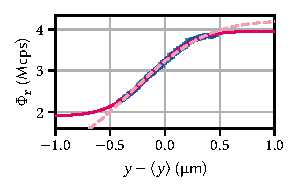
\includegraphics{img/pdf/setup/knife_edge_erf}
    \caption[\imgsource{img/py/setup/vibration_spectroscopy.py}]{
        Reflectance gradient of the edge of a \ch{Au} gate electrode on the bare \ch{GaAs} surface.
        The dashed line is a fit to \cref{eq:setup:knife_edge} with $\reflectance_0$ fixed while the solid includes this parameter in the fit.
    }
    \label{fig:app:setup:vibrations:knife_edge}
\end{marginfigure}

From the refractive index of \ch{GaAs}, we would expect
\begin{equation}
    \reflectance_0 = \abs{\frac{n-1}{n+1}}^2 \approx \qty{32}{\percent}
\end{equation}
at zero temperature~\cite{Talghader1995}.
\Cref{fig:app:setup:vibrations:knife_edge} shows the same data as \cref{fig:setup:vibrations:calibration:pos_vs_cps} together with fits to \cref{eq:setup:knife_edge} in magenta.
The dashed line is a fit with $\reflectance_0$ fixed, whereas the solid line is a fit including $\reflectance_0$ as a free parameter.
Clearly, the latter matches the data better, resulting in
\begin{align}
    \reflectance_0 &= \qty{65.1+-1.4}{\percent} \\
    w_0 &= \qty{0.624+-0.028}{\micro\meter}.
\end{align}
The discrepancy in reflectance might be explained by multilayer and thin-film effects given that the sample is only \qty{220}{\nano\meter} thick and warrants closer investigation.
More likely, the assumption that the \ch{Au} optical gate is perfectly reflecting is to be challenged as its thickness corresponds to only a fifth of the wavelength.
In \cref{part:exp}, I carry out \gls{tmm} simulations to this end.
% TODO: Adapt conditioned on TMM simulation results.
The Gaussian beam waist radius $w_0$ resulting from the fit is in quite good agreement with the results obtained in \cref{subsec:setup:optics:coupling:imaging}, where I obtained the value \qty{0.60}{\micro\meter} and \qty{0.84}{\micro\meter} for the $y$- and $z$-direction, respectively (see \cref{tab:setup:optics:coupling:imaging}, but note the different coordinate systems).
